\documentclass[../main.tex]{subfiles}
\begin{document}
\chapter{Introduction}\label{chapter1}
\section{Neutron Stars}\label{section:neutron_stars}
Neutron stars are some of the most interesting and exotic objects in the Universe.  With a mass slightly larger than that of the Sun and the size of a city, they are made up of matter denser than anything that can be found on Earth.  As such, they provide a unique way to probe dense matter physics, even from thousands of light years away.  Indeed, these stars have been observed in both radio and X-rays since the 1960's \citep{Hewish1968,Shklovsky1967}.  These observations have so far led to constraints on parameters such as surface temperature, atmospheric composition and spin frequency of these stars. However, much is still not well understood about neutron stars. Most notably, the dense matter equation of state is still unknown. A lot of work, both theoretical and observational, is dedicated to finding masses and radii of neutron stars in order to constrain this equation of state.
 
We now live in a golden age of neutron star astronomy, with the detection of double neutron star mergers with gravitational waves \citep{Abbott2017}, the launch of modern X-ray observatories designed to study neutron stars and, as as result, the first reliable neutron star radius measurements \citep{Gendreau2017,Miller2019}. On the theoretical side, there is still a lot of room for improvement in the physical models that describe various phenomena happening in neutron stars. A type of system where we can study neutron stars are X-ray binaries, where a neutron star accretes from a companion star. Accreted H/He fuel periodically burns on the neutron star surface, making the neutron star very bright, and giving an opportunity to study the neutron star directly. These systems are the focus of this thesis, where we study the ejection of matter in bright thermonuclear bursts. %We begin, in this introduction, by presenting the general theory and open questions surrounding neutron star thermonuclear bursts and radius expansion.

% One such phenomenon is the expansion of the neutron star apparent radius, which is thought to be driven by winds following thermonuclear bursts occurring on the stellar surface. The subject of this thesis is the improvement of models of this radius expansion and the outflows that are driving it. We begin, in this introduction, by presenting the general theory and open questions surrounding neutron star thermonuclear bursts and radius expansion.
 
 
 %In particular, the equation of state (EOS) of the dense matter that makes up neutron stars is still unknown.  This fundamental relation is what links the state variables (temperature, pressure, density) to each other, and is essential to understand complex phenomena such as double neutron-star mergers, which have recently been observed for the first time with gravitational waves \citep{Abbott2017}.  This makes the neutron star EOS one of the most sought after quantities in physics today.  While many EOS's have been proposed \citep{Ozel2016a}, it is not yet possible to determine which is correct.  Fortunately, there is  a way to do this using observations.  If we can determine the radius of neutron stars with a range of different masses, we can place constraints on which EOS's are possible, since every equation predicts different radii for any given mass.  This approach has been tried and tested a lot by the astronomy \& astrophysics community in the last decade, and has already lead to promising results \citep{Ozel2016a}. But to obtain a final answer, progress in two areas has to be made: observations and theoretical models.  The work of this thesis slots into the second category. 
 
 %\textbf{make second paragraph stand on its own. tone down eos. Somethign else?? I guess introduce what this project is about}
 
\section{Type I X-ray bursts}\label{section:type_I_xray_bursts}
Neutron stars are sometimes found in binary systems where they orbit another star with a period of hours to days \citep{Lewin1993}. In this configuration, when the companion star begins expanding as it goes through its main sequence evolution, it is possible for its outer layers to escape its surface and funnel onto the surface of the neutron star in a process called \textit{accretion}.  As matter builds up on top of the neutron star crust, it eventually reaches a critical pressure where helium quickly fuses via the triple-$\alpha$ process.  The star cannot compensate for this sudden release of heat by cooling, thus creating a thermonuclear runaway, which quickly spreads through the whole ocean and burns most of the hydrogen and helium. This event results in the neutron star shining brightly in X-rays for seconds to minutes. This X-ray flash is referred to as a \textit{Type I X-ray burst}, or \textit{burst} for short. A typical burst light curve is shown in Fig.~\ref{fig:keek2018_fig3}. 

Some bursts reach luminosities so high that radiation pressure starts to push some of the accreted material outward, making the star temporarily appear bigger and colder due to the expansion of the photosphere.  These \textit{photospheric radius expansion} (PRE) bursts are observed as near blackbodies with a temperature of ${\sim}1$ keV at the burst peak, and ${\sim}1-5$ keV when the photosphere touches back down to the surface. The light curve shown in the top panel of Fig.~\ref{fig:keek2018_fig3} is from such a PRE burst, with the bottom two panels showing best fit values for the blackbody temperature and emitting radius. The PRE phase of the burst is marked by the concurrent drop in temperature and jump in radius.  

\begin{figure}[htb!]
    \centering
    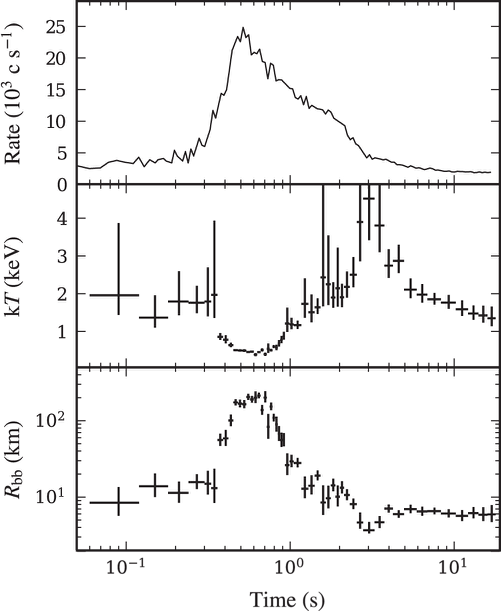
\includegraphics[width=0.65\textwidth]{figures/Keek2018_fig3_mod.png}
    \caption[Type I X-ray burst light curve]{Light curve (top panel) and blackbody fits (second and third panels) from a Type I X-ray burst in the low-mass X-ray binary 4U 1820-30, observed by \textit{NICER} in august 2017. Adapted from \citet{Keek2018a}.}
    \label{fig:keek2018_fig3}
\end{figure}

%\textbf{before Nicer paragraph, talk about all the bursts seen by rxte (catalog paper). Sometimes very little expansion, sometimes large. Int zand wegberg paper super expansion : shell? Timescales question. How does the burst evolve from hydrostatic to wind? Maybe add 3hour burst fig.}

A large number of type I X-ray bursts have been observed from a multitude of systems since their discovery in 1976 \citep{Grindlay1976}. More than a thousand bursts have been observed by the Rossi X-ray Timing Explorer (RXTE) alone \citep{Galloway2008}. In this catalogue, 35 of the 48 bursting sources have had PRE bursts observed. An intriguing puzzle is the fact that there are seemingly two categories of radius expansion. In most cases, the photosphere only expands to tens of kilometres above the stellar surface. In the rare \textit{superexpansion} bursts, the photosphere surpasses a thousand kilometres in radius \citep{IntZand2010}. It has been suggested that the second case could be caused by the wind-driven ejection of a geometrically thin shell which remains optically thick until it has expanded and cooled enough at large radii. This raises questions about the timescales of the expansion, and the manner in which the initially hydrostatic envelope can transition into a fully outflowing wind. 

The burst shown in Fig.~\ref{fig:keek2018_fig3}, which occured in August 2017 in the low-mass X-ray binary 4U 1820-30, marked an important moment in the field of Type I X-ray bursts as it was the first PRE burst observed by the \textit{Neutron Star Interior Composition Explorer} (\Nicer), an X-ray observatory on the International Space Station that was launched in 2017 \citep{Gendreau2017}.  \Nicer's principal objective is to constrain the dense matter equation of state by obtaining mass and radius measurements of neutron stars.  To accomplish this goal, NICER needs a wide spectral range, especially in the soft (${<}1$ keV) band. This makes NICER the best tool yet to observe PRE bursts, as it can track the whole evolution of the photospheric radius \citep{Keek2018a}.  Indeed, previous X-ray instruments that had no soft response would observe an artifical dip in total luminosity, as the blackbody temperature would exit their spectral range. This contrast between {\Nicer} and previous telescopes can be seen in figure \ref{fig:keek2018_fig1}. 

\begin{figure}[htb!]
    \centering
    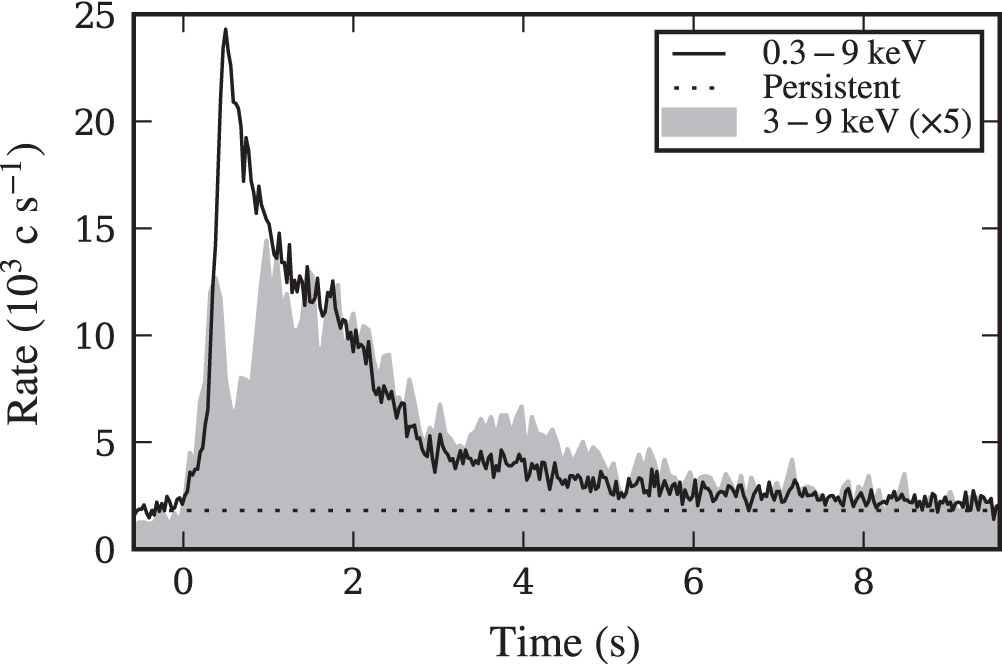
\includegraphics[width=0.65\textwidth]{figures/Keek2018_fig1_mod.jpg}
    \caption[\Nicer~ PRE burst light curve]{Light curve from a Type I X-ray burst in 4U 1820-30 considering different spectral ranges of observation. The solid line shows the count rate in the {\Nicer} spectral range, while the gray shaded area shows the count rate (scaled up by a factor of 5) for instruments with no soft X-ray response. The dotted line shows the count rate for the persistent (pre-burst) emission. Adapted from \citet{Keek2018a}.}
    \label{fig:keek2018_fig1}
\end{figure}

\section{Open questions}\label{sec:open_questions}
There has been, in the past few years, a renewed interest in theoretical models of the outflows driving the PRE phase, marked for example by the works of \citet{YuHangWeinberg2018} and \citet{Herrera2020}. These have certainly been motivated in large part by the arrival of \Nicer, and the opportunity for theorists and observers to work together to answer a number of open questions regarding Type I X-ray bursts. We highlight two of these major open questions here. \\

\noindent\textbf{Can heavy elements produced in the nuclear reaction networks at the onset of the burst be ejected during the subsequent outflows?} 

%\textbf{Bursts are a really unique environment for nuclear burning because of rp-process. Burning helium with a lot of hydrogen (protons) present. Maybe put this at the beginning of the first open question?}

Type I X-ray bursts are a unique environment for nuclear burning, as helium is being burned with a large number of protons from ionized hydrogen present. Via the rapid proton capture (rp) process, many heavy elements, even  far beyond the iron group, are produced in a short time frame \citep{Schatz1999}. There has recently been mounting observational evidence, in the form of spectral edges and lines within Type I X-ray burst spectra \citep{IntZand2010,Kajava2017,Strohmayer2019}, that heavy elements such as iron and nickel are present at the photosphere during the expansion phase. This suggests that nuclear ashes are somehow dredged up, possibly via convection, and subsequently lifted up during the expansion. If a wind is driving the expansion, it is possible that these heavy elements are completely ejected from the star and deposited into the accretion disk, or even into the interstellar medium.  

The conditions and manner in which these ashes can be lifted is not well understood, and neither is the expected observational signature of heavy elements if they are truly present in the outflow. However, recent results from \Nicer {} data and presented in \citet{Strohmayer2019} show some promise for the latter. In the days following the burst from 4U 1820-30, shown in Fig.~\ref{fig:keek2018_fig3} and \ref{fig:keek2018_fig1}, three more bursts exhibiting a PRE phase were observed. Among these four, blackbody fits of the spectra revealed that two of the bursts had expansion phases with a photosphere of ${\sim}100$ km, while the other two had weaker expansion, with a photosphere of ${\sim}75$ km. By co-adding spectra of the bursts within each pair and fitting these with an absorbed blackbody model, it became clear that the bursts had spectral lines in their spectra, of both emission and absorption nature. This can be seen in Fig.~\ref{fig:strohmayer_burstpair_residuals}. Further, the spectral shift between the two pairs is the same for each line, with weaker burst lines appearing \textit{redshifted} compared to the other ones by a factor of 1.046. This is consistent with the lines being produced in a wind. Indeed, the lines in the weaker bursts should be produced closer to the neutron star, and thus have stronger redshift. On top of this effect, wind models, which we will discuss in the next section, show that stronger bursts have larger wind velocities, which means the lines are more \textit{blueshifted}. \citet{Strohmayer2019} argue that both of these effects work together to create the spectral shifts seen in Fig.~\ref{fig:strohmayer_burstpair_residuals}. While this represents quite a convincing argument for the existence of both burst-driven winds and heavy element ejection, it suffers from the lack of theoretical models of such winds, especially ones which include a heterogeneous gas composition with heavy materials, which are required to provide values for the emission radii and velocities of these lines. \\

% \begin{figure}[htb!]
%     \centering
%     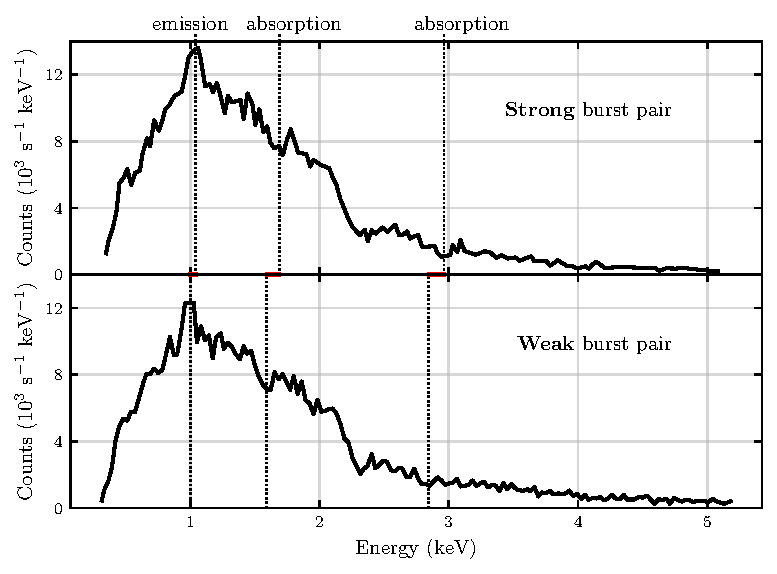
\includegraphics[width=0.9\textwidth]{figures/Strohmayer2019_burstpair_lines.pdf}
%     \caption[Co-added spectra of two pairs of bursts]{Co-added spectra of two pairs of bursts in 4U 1820-30 observed by \Nicer. \textit{Top (bottom)}: Bursts with strong (weak) expansion, i.e a large (small) photosphere and small (high) blackbody temperature. Dotted lines indicate the centroid position of the emission and absorption lines, found from residuals of the absorbed blackbody fits. Data points and line energies are taken directly from \citet{Strohmayer2019}.}
%     \label{fig:strohmayer_burstpair_lines}
% \end{figure}

\begin{figure}[htb!]
    \centering
    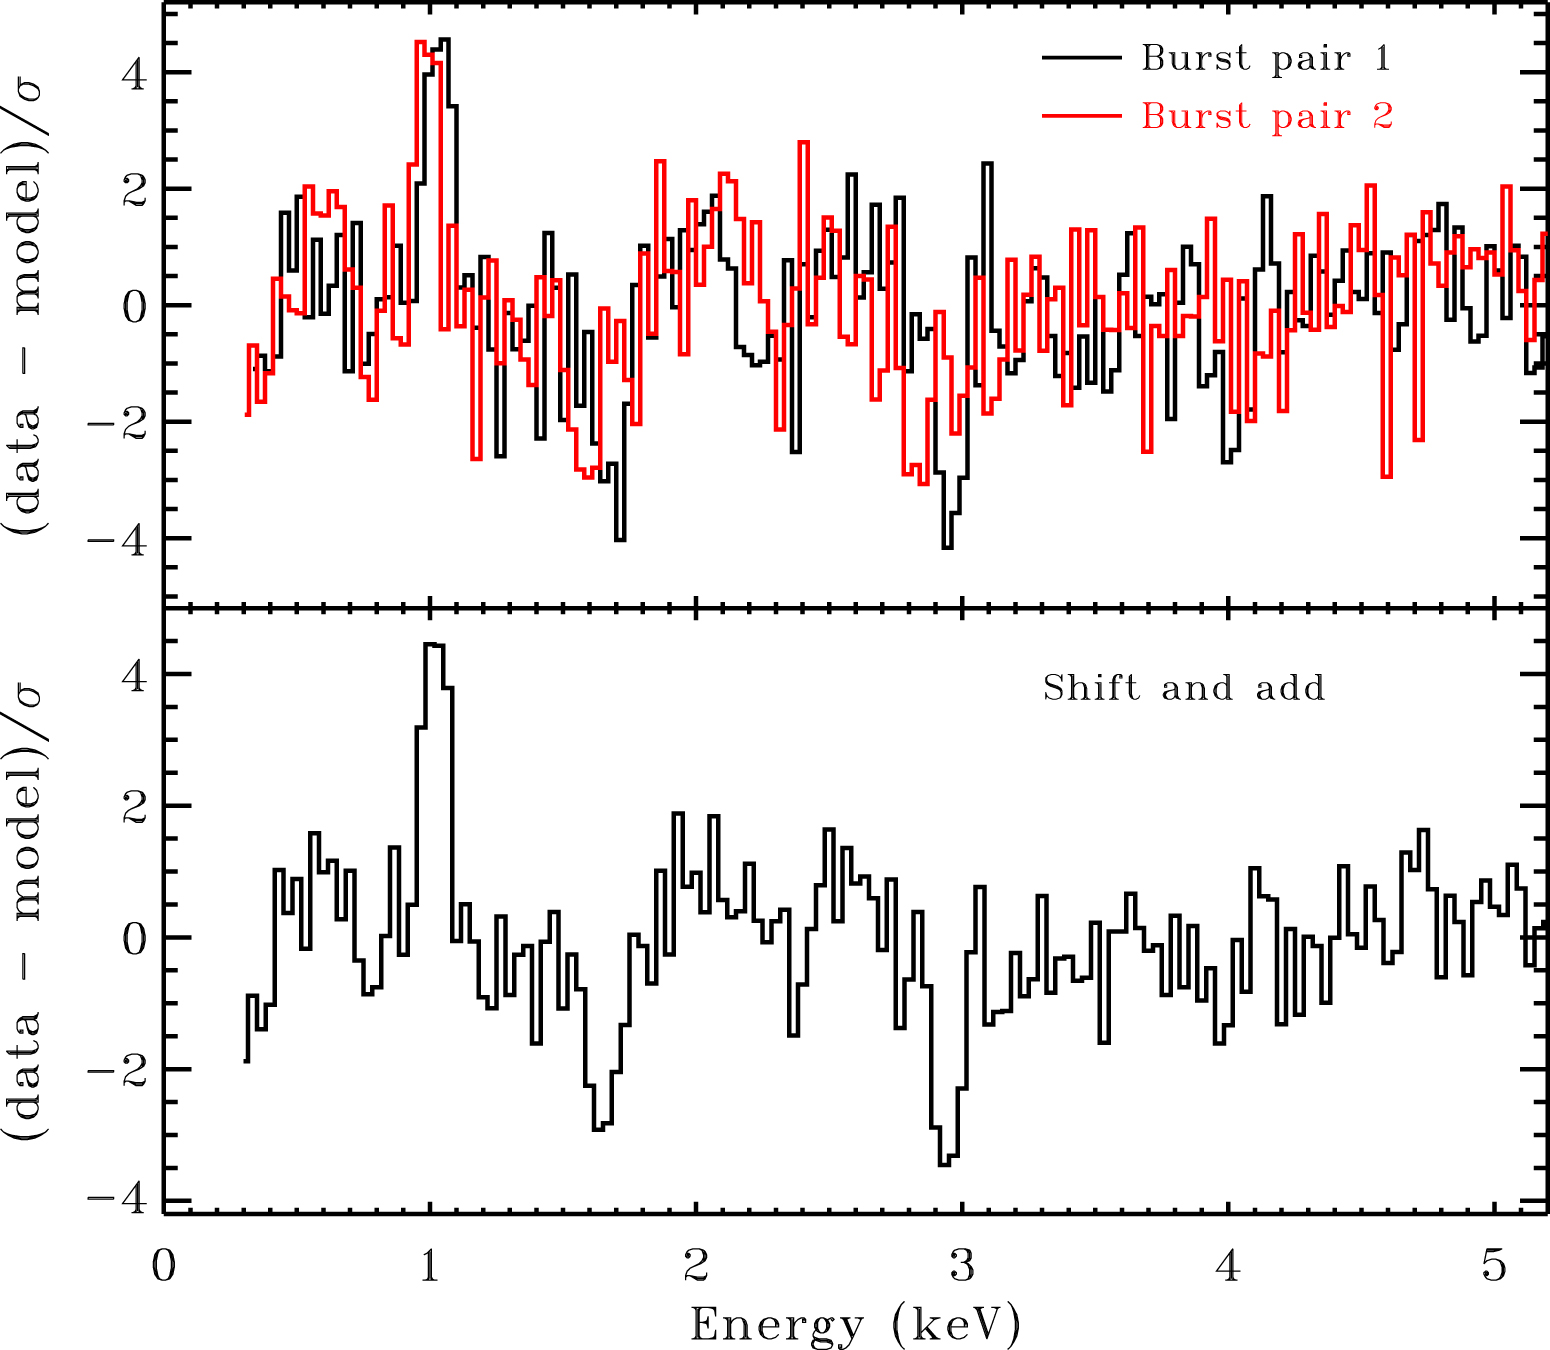
\includegraphics[width=0.8\textwidth]{figures/Strohmayer2019_residuals.jpg}
    \caption[Burst spectra fit residuals showing spectral lines]{Fit residuals of the absorbed blackbody model for the stronger (pair 1) and weaker (pair 2) bursts. In the bottom panel, the residuals are added after the pair 2 residuals have been shifted by the best fitting line ratio of 1.046. From \citet{Strohmayer2019}.}
    \label{fig:strohmayer_burstpair_residuals}
\end{figure}

\noindent\textbf{What is the time-dependent evolution of the photosphere during the PRE phase, and how does it vary from burst to burst?} 

%The aforementioned blackbody fits to burst spectra obviously come with the presupposition that burst spectra are indeed planckian, which has been challenged in the past \citep{VanParadijs1982,Titarchuk1994}.
This question is especially relevant now with the availability of \Nicer {} data, which allows us to track the temperature throughout the expansion phase, and determine the emission radius with blackbody fits, as shown in Fig.~\ref{fig:keek2018_fig3}. An important way in which this has been used is to label the peak of the blackbody temperature curve, after the expansion phase, as the \textit{touchdown} point, i.e the moment where the atmosphere collapses back down to the surface and the photosphere (which still presumably emits as a blackbody) is equal to the neutron star radius. For example in Fig.~\ref{fig:keek2018_fig3}, the touchdown point is at 30s. Using this and independent measurements of the neutron star mass, $M$-$R$ constraints have been placed on the neutron star equation of state \citep{Ozel2016a}.  

It is not clear however if this method is truly valid, as the systematics of the photosphere evolution and touchdown point are not well understood, as was first pointed out by \citet{Steiner2010}. One possible scenario in which the touchdown interpretation would be incorrect is one in which the atmosphere does not collapse to the surface right after the main expansion phase, but rather remains slightly expanded above the surface, sustained by a still substantial burning layer flux. It would then slowly fall back down to the surface as the neutron star cools. The true touchdown point could therefore be much later than the PRE phase, far into the tail of the burst light curve, at which point the emission might not be planckian. Therefore, more work needs to be done to model the evolution of the photosphere, and how it relates to the observables, mainly the total luminosity and effective temperature of the spectra, as a function of time. 

Another reason why it is important to understand these systematics is that PRE bursts are often used as standard candles to determine the distance to neutron stars. This is done by assuming that the luminosity at the photosphere is the critical luminosity, which we will introduce in the next section, and relating it to the peak flux seen at the telescope by a factor $4\pi d^2$, assuming spherical emission \citep{Galloway2008}. While it has been shown, using sources with independently constrained distances, that many PRE bursts were indeed good standard candles (e.g. by \citet{Kuulkers2003}), significant deviations in some sources indicate that the assumptions do not always hold.


\section{Basic theory and previous theoretical work}\label{section:basic_theory}
For a burst to exhibit PRE, a high enough luminosity must be attained in order to break hydrostatic equilibrium. The critical luminosity can be found by equating gravity and radiation pressure.  Far from the star, where temperatures are low enough that the opacity is from Thomson scattering, this leads to the classical \textit{Eddington luminosity},
\begin{equation}\label{eq:LEdd}
    \Ledd = \frac{4\pi GMc}{\kappa_0}\,,
\end{equation}
where $M$ is the mass of the star and $\kappa_0=0.2(1+X)$ g cm$^{-2}$ is the constant electron scattering opacity, where $X$ is the hydrogen fraction.

Close to the star, at a distance $r$ from the center, this changes in two ways. If we consider general relativity, then the local effective gravity is increased over the Newtonian value by a factor related to the space-time metric we choose to use. We will consider the Schwarzschild metric, which describes the space-time surrounding a central non-rotating object. Also, in general, radiation interacts with the gas in ways that depend on both its density $\rho$ and temperature $T$. This must be reflected by a non-constant opacity. The \textit{local critical luminosity} is therefore
\begin{equation}\label{eq:Lcrit}
    \Lcr=\frac{4\pi GMc}{\kappa(\rho,T)}\left(1-\frac{2GM}{rc^2}\right)^{-1/2}\,.
\end{equation}
At large radii, the temperature and density are small and the opacity goes to the constant $\kappa_0$, such that $\Lcr\rightarrow \Ledd$. General relativity also has the effect of differentiating the observed luminosity between different observers.  If the local luminosity is $L$, the luminosity seen by an observer at infinity is
\begin{equation}\label{eq:Linf}
    \Linf=L\left(1-\frac{2GM}{rc^2}\right)\,.
\end{equation}
There are two metric terms here, one for time dilation which makes photons come out at a slower rate, and another for redshift, which lowers the total energy of the radiation field.  


The temperature dependence of the opacity is significant in the context of bursts, since at high temperatures, when electrons reach relativistic velocities and photon collisions become subject to inelastic Compton scattering, the electron scattering opacity is drastically reduced. \citet{Paczynski1983} gives the following interpolation formula
\begin{equation}\label{eq:kappa}
    \kappa(T)=\kappa_0 \left[1+\left(\frac{T}{4.5\times 10^8 \text{ K}}\right)^{0.86}\right]^{-1}\,,
\end{equation}
based on tabulated values of \citet{Buchler1976}. In bursts, temperatures of over $10^9$ K are readily attained. This creates a situation where the luminosity can be very high, even \textit{super-Eddington} (referring to Eq.~\ref{eq:LEdd}), while at the same time being \textit{sub-critical} (referring to Eq.~\ref{eq:Lcrit}). The atmosphere can still expand, even in the sub-Eddington case, because any luminosity causes an outward radiation pressure which reduces the effective gravity
\begin{equation}\label{eq:geff}
    g_\text{eff}=g\left(1-\frac{L}{\Lcr}\right)\,.
\end{equation}
So the temperature dependence of the opacity already reveals the structure of the outflows; we expect a compact, geometrically thin envelope in hydrostatic equilibrium that gradually transitions into an extended region of gas as $T$ and $\Lcr$ drop, allowing the photons to ``push'' the gas more effectively. 

But when discussing this luminosity driven expansion of the atmosphere, we are actually talking about two possible regimes, which are illustrated in Fig.~\ref{fig:diagram}. The first, most well-known case, is the \textit{super-Eddington wind} regime, which will inevitably occur if $L^\infty>\Ledd$. This inequality implies mass loss because the luminosity is greater than Eddington all the way out to infinity, where matter must be flowing in all the way from the star. The excess photon energy must be used to unbind accreted material, giving the approximate relation
\begin{equation}
    \frac{dM}{dt}\approx \frac{L^\infty-\Ledd}{GM/R}\,.
\end{equation}
Super-Eddington winds are ubiquitous in massive stars, where the main driving mechanism is kinetic energy deposition (see for reference \citet{Quataert2016}).  These burst super-Eddington winds however are radiation pressure driven, i.e it is the photons, trapped in the optically thick fluid, that transfer their energy as they diffuse through the gas. Therefore, these winds are extremely sensitive to the exact temperature dependent scattering opacity, which is not the case for massive stellar winds as per \citet{Quataert2016}. 

The wind regime has been studied extensively in the past. Many papers in the 1980's demonstrated calculations of steady-state wind solutions, starting with \citet{Ebisuzaki1983} and \citet{Kato1983a}, who solved time-independent Newtonian hydrodynamics and optically thick radiative transfer equations with different assumptions and approximations.  Various improvements were made in later years, such as a transition into optically thin regions \citep{Quinn1985}, the inclusion of general relativity \citep{Paczynski1986b} and more detailed radiative transfer \citep{Joss1987,Nobili1994}.  More recently, \citet{YuHangWeinberg2018} performed time-dependent calculations of winds for the first time, going back to Newtonian gravity and pure optically thick radiative transfer, but with a focus on tracking the composition of different elements over time and space.  The different approximations made by these various papers are summarized in Table \ref{tab:literature}, which shows that there clearly needs to be more work done to include all of these different effects in the same calculation.

\begin{table}[ht!]
    \centering
    \caption{Previous work on burst super-Eddington winds}
    \vspace*{3mm}
    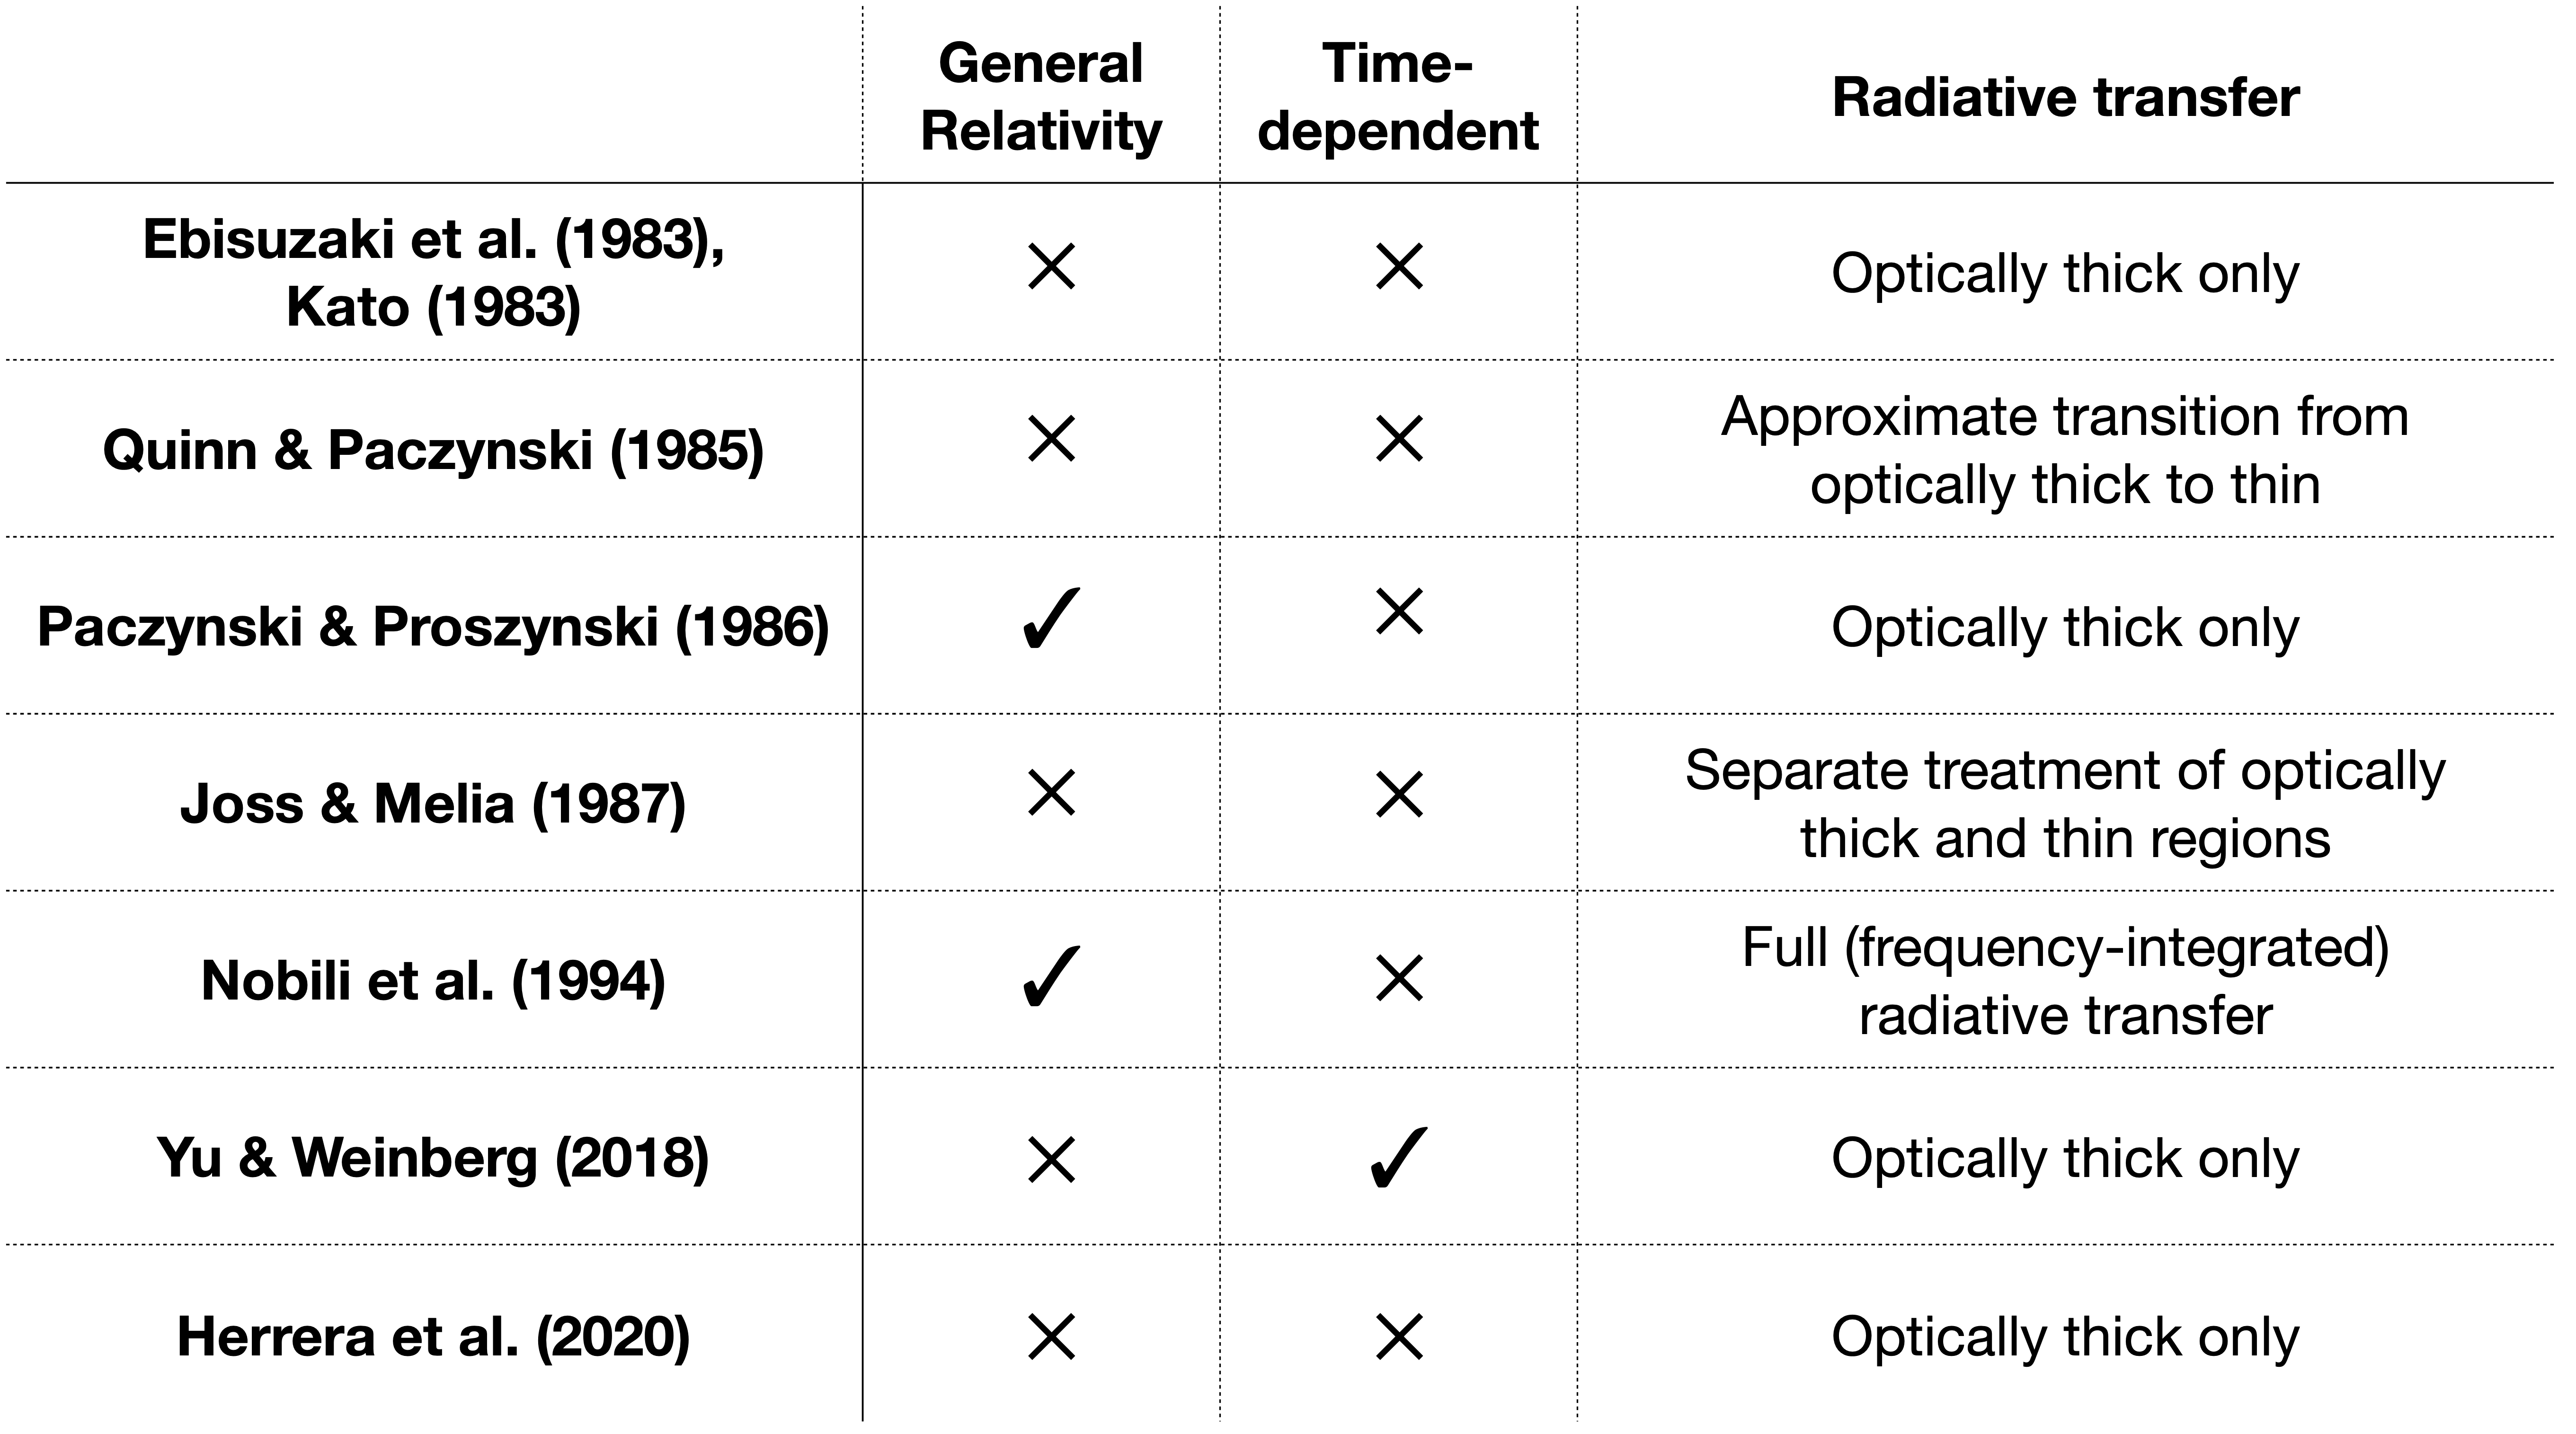
\includegraphics[width=0.8\textwidth]{figures/table.png}
    \label{tab:literature}
\end{table}

The second, less discussed regime, is the \textit{expanded envelope} in hydrostatic equilibrium, which occurs when $L^\infty \lesssim \Ledd$. With a smaller luminosity, the surface temperature is smaller than in the wind case, such that $L$ is in fact closer to $\Lcr$ than in the wind case, triggering expansion given the effective gravity in Eq.~\eqref{eq:geff}. Since there is no mass loss and no velocity, there is no net transfer of energy from the photons to the gas. Therefore, the luminosity $L^\infty$ is in this case a constant throughout the model. The local luminosity, however, is a function of radius, according to Eq.~\eqref{eq:Linf}. The expansion will self-adjust such that $L\lesssim \Lcr$ at every radius in order to maintain hydrostatic equilibrium. In fact, this expanded envelope regime is a general relativistic effect, as the redshift-dependent luminosity is a requirement for maintaining equilibrium. This was explained by \citet{Paczynski1986a}, the only paper in the literature discussing relativistic expanded envelopes in relation to Type I X-ray bursts, who pointed out that previous attempts to model envelopes without general relativity (or without temperature dependent opacity) were incorrect, and that they could only produce very compact envelopes, not the extended ones that appear with the inclusion of redshift.

\section{Outline}\label{section:outline}

%\textbf{Don't undersell. We want to make progress in the models to get closer to answering all the questions layed out earlier. We're making a sequence of fully consistent models. Grid of models as an outer boundary condition for time dependent codes. }

The objective of this work is to improve radius expansion models to help answer many of the questions that were presented in this introduction. We have created a sequence of fully consistent envelope and steady-state wind models that can be linked to the state of the burning layer at any point during the burst evolution. These models can be used as an outer boundary condition in time-dependent codes simulating the burning layer, as well as guides to interpret data from the large number of catalogued observations. For the first time, we can also compare the two expansion regimes to each other and analyze the transition between the two in a real burst. 

%Never before have the two expansion  regimes discussed in the previous section been compared to each other. The aim of this work is to calculate steady-state wind and expanded envelope models with self-consistent input physics and assumptions, then analyze them together, linking the main observables (observed luminosity, photospheric radii and temperatures) to the state of the burning layer (base luminosity, temperature and density) at any given time in the evolution of the bursts. 

We begin with a derivation of the equations of radiation hydrodynamics used throughout this work in Chapter 2, then describe the numerical method and show the results for the wind models in Chapter 3, and expanded envelope models in Chapter 4. Finally, we compare the two regimes and make final remarks on the use of these stationary solutions to describe the dynamics of different parts of PRE bursts in Chapter 5.

\begin{figure}[htb!]
    \centering
    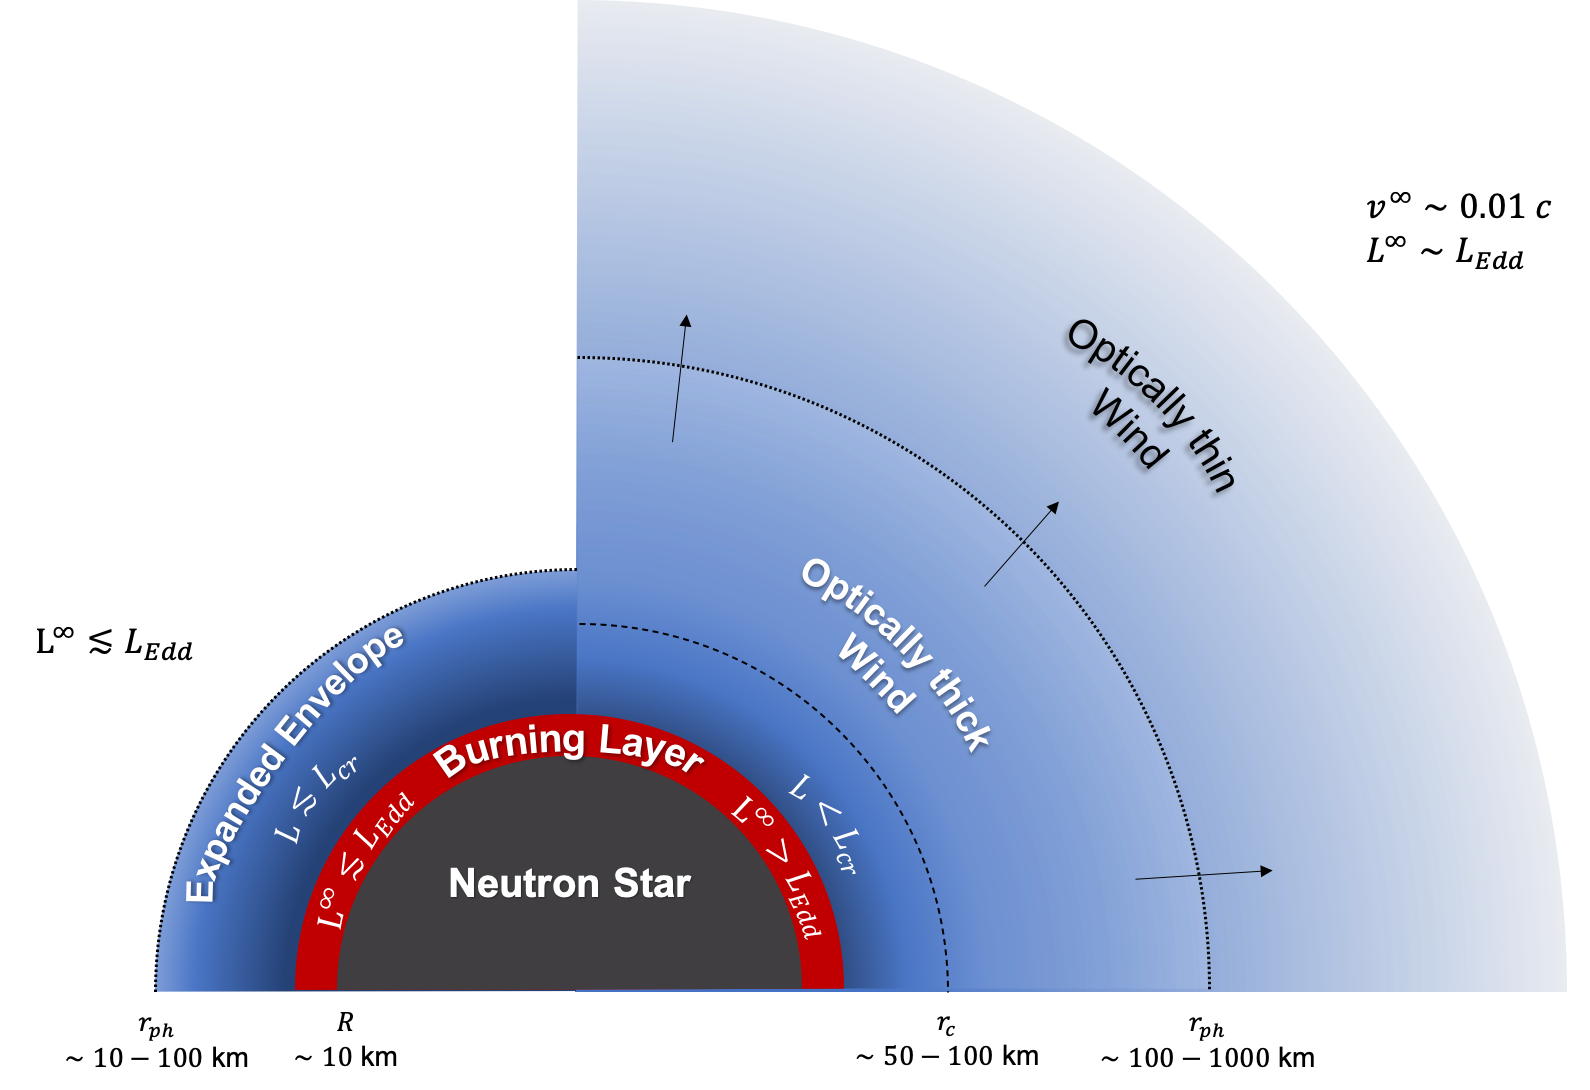
\includegraphics[width=\textwidth]{figures/diagram.png}
    \caption[Diagram of PRE burst expansion regimes]{Diagram summarizing the relevant quantities in the two PRE burst expansion regimes. We explain the definitions for the critical point $r_c$ and photospheric radius $r_\text{ph}$ and how to calculate solutions to these structures in Chapter 3 (winds) and Chapter 4 (envelopes).}
    \label{fig:diagram}
\end{figure}

\biblio

\end{document}